%%% demothesis.tex ---
%%
%% Filename: demothesis.tex
%% Description:
%% Author: Ola Leifler
%% Maintainer:
%% Created: Thu Oct 14 12:52:20 2010 (CEST)
%% Version: $Id$
%% Version:
%% Last-Updated: Thu Apr 20 20:49:56 2017 (+0200)
%%           By: Ola Leifler
%%     Update #: 166
%% URL:
%% Keywords:
%% Compatibility:
%%
%%%%%%%%%%%%%%%%%%%%%%%%%%%%%%%%%%%%%%%%%%%%%%%%%%%%%%%%%%%%%%%%%%%%%%
%%
%%% Commentary:
%%
%%
%%
%%%%%%%%%%%%%%%%%%%%%%%%%%%%%%%%%%%%%%%%%%%%%%%%%%%%%%%%%%%%%%%%%%%%%%
%%
%%% Change log:
%%
%%
%% RCS $Log$
%%%%%%%%%%%%%%%%%%%%%%%%%%%%%%%%%%%%%%%%%%%%%%%%%%%%%%%%%%%%%%%%%%%%%%
%%
%%% Code:

\documentclass[msc,lith,english]{liuthesis}
%% Settings go in settings.tex
%%% settings.tex ---
%%
%% Filename: settings.tex
%% Description:
%% Author: Ola Leifler
%% Maintainer:
%% Created: Tue Oct 19 21:11:31 2010 (CEST)
%% Version: $Id$
%% Version:
%% Last-Updated: Tue Apr 25 08:49:48 2017 (+0200)
%%           By: Ola Leifler
%%     Update #: 43
%% URL:
%% Keywords:
%% Compatibility:
%%
%%%%%%%%%%%%%%%%%%%%%%%%%%%%%%%%%%%%%%%%%%%%%%%%%%%%%%%%%%%%%%%%%%%%%%
%%
%%% Commentary:
%%
%%
%%
%%%%%%%%%%%%%%%%%%%%%%%%%%%%%%%%%%%%%%%%%%%%%%%%%%%%%%%%%%%%%%%%%%%%%%
%%
%%% Change log:
%%
%%
%% RCS $Log$
%%%%%%%%%%%%%%%%%%%%%%%%%%%%%%%%%%%%%%%%%%%%%%%%%%%%%%%%%%%%%%%%%%%%%%
%%
%%% Code:

\usepackage[backend=biber,hyperref,giveninits=true]{biblatex}
%% To set the font of your thesis, use the \setmainfont{} command,
%% surrounded with \ifxetex if you want to switch between xelatex and pdflatex
\ifxetex
%\setmainfont [Scale=1]{Georgia}
\fi

%%%%%%%%%%%%
%% The VZ43 chapter style, from Memoir contributed chapter styles: ftp://ftp.tex.ac.uk/ctan%3A/info/MemoirChapStyles/MemoirChapStyles.pdf
%%%%%%%%%%%

\usepackage{calc,color}
\newif\ifNoChapNumber
\newcommand\Vlines{%
\def\VL{\rule[-2cm]{1pt}{5cm}\hspace{1mm}\relax}
\VL\VL\VL\VL\VL\VL\VL}
\makeatletter
\setlength\midchapskip{0pt}
\makechapterstyle{VZ43}{
\renewcommand\chapternamenum{}
\renewcommand\printchaptername{}
\renewcommand\printchapternum{}

\renewcommand\chapnumfont{\Huge\bfseries\centering}
\renewcommand\chaptitlefont{\Huge\bfseries\raggedright}
\renewcommand\printchaptertitle[1]{%
% \Vlines\hspace*{-2em}%
\begin{tabular}{@{}p{1cm} p{\textwidth-3cm}}%
\ifNoChapNumber\relax\else%
\colorbox{black}{\color{white}%
\makebox[.8cm]{\chapnumfont\strut \thechapter}}
\fi
& \chaptitlefont ##1
\end{tabular}
\NoChapNumberfalse
}
\renewcommand\printchapternonum{\NoChapNumbertrue}
}
\makeatother


%% To set bibliography options, refer to the biblatex manual and use
%% the ExecuteBibliographyOptions command below to set your options

\ExecuteBibliographyOptions{maxnames=99}


%% Change this to your appropriate BibTeX reference file (.bib)

\addbibresource{references.bib}

%%%%%%%%%%%%%%%%%%%%%%%%%%%%%%%%%%%%%%%%%%%%%%%%%%%%%%%%%%%%%%%%%%%%%%
%%% settings.tex ends here

%%% Local Variables:
%%% mode: latex
%%% TeX-master: "demothesis"
%%% End:

\usepackage{rotating}
\usepackage{color}

\usepackage{xargs}                      % Use more than one optional parameter in a new commands
% \usepackage[pdftex,dvipsnames]{xcolor}  % Coloured text etc.
\usepackage[colorinlistoftodos,prependcaption,textsize=tiny]{todonotes}

\newcommandx{\unsure}[2][1=]{\todo[linecolor=red,backgroundcolor=red!25,bordercolor=red,#1]{#2}}
\newcommandx{\change}[2][1=]{\todo[linecolor=blue,backgroundcolor=blue!25,bordercolor=blue,#1]{#2}}
\newcommandx{\source}[2][1=]{\todo[linecolor=orange,backgroundcolor=orange!25,bordercolor=orange,#1]{#2}}
\newcommandx{\info}[2][1=]{\todo[linecolor=OliveGreen,backgroundcolor=OliveGreen!25,bordercolor=OliveGreen,#1]{#2}}
\newcommandx{\improvement}[2][1=]{\todo[linecolor=Plum,backgroundcolor=Plum!25,bordercolor=Plum,#1]{#2}}
\newcommandx{\thiswillnotshow}[2][1=]{\todo[disable,#1]{#2}}

% \usepackage{changebar}

\department{Institutionen för teknik och naturvetenskap}
\departmentenglish{Department of Science and Technology}
\departmentshort{ITN}

\externalsupervisor{Alexander Bock}
\supervisor{Emil Axelsson}
\examiner{Anders Ynnerman}
\titleenglish{Developing a Web GUI \\for rapid prototyping \\and public exhibitions}
\subtitleenglish{An OpenSpace project}
\titleswedish{Utveckling av ett GUI-ramverk med webbtekniker}
\thesissubject{Datateknik}

\publicationyear{2017}
\currentyearthesisnumber{???}
% TODO: Fix publication date
\dateofpublication{2017-05-10}

\author{Klas Eskilson}

\begin{document}

\listoftodos[Notes]
\newpage

\chapterstyle{VZ43}

%%% Intro.tex ---
%%
%% Filename: Intro.tex
%% Description:
%% Author: Ola Leifler
%% Maintainer:
%% Created: Thu Oct 14 12:54:47 2010 (CEST)
%% Version: $Id$
%% Version:
%% Last-Updated: Thu May 19 14:12:31 2016 (+0200)
%%           By: Ola Leifler
%%     Update #: 5
%% URL:
%% Keywords:
%% Compatibility:
%%
%%%%%%%%%%%%%%%%%%%%%%%%%%%%%%%%%%%%%%%%%%%%%%%%%%%%%%%%%%%%%%%%%%%%%%
%%
%%% Commentary:
%%
%%
%%
%%%%%%%%%%%%%%%%%%%%%%%%%%%%%%%%%%%%%%%%%%%%%%%%%%%%%%%%%%%%%%%%%%%%%%
%%
%%% Change log:
%%
%%
%% RCS $Log$
%%%%%%%%%%%%%%%%%%%%%%%%%%%%%%%%%%%%%%%%%%%%%%%%%%%%%%%%%%%%%%%%%%%%%%
%%
%%% Code:


\chapter{Introduction}
\label{cha:introduction}

The introduction shall be divided into these sections:

\section{Motivation}
\label{sec:motivation}

This is where the studied problem is described from a general
point of view and put in a context which makes it clear that
it is interesting and well worth studying. The aim is to make
the reader interested in the work and create an urge to
continue reading.

\section{Aim}
\label{sec:aim}


What is the underlying purpose of the thesis project?

\section{Research questions}
\label{sec:research-questions}


This is where the research questions are described.
Formulate these as explicit questions, terminated with a
question mark. A report will usually contain several different
research questions that are somehow thematically connected.
There are usually 2-4 questions in total.

Examples of common types of research questions (simplified
and generalized):

\begin{enumerate}
\item How does technique X affect the possibility of achieving the
  effect Y?

\item How can a system (or a solution) for X be realized so
  that the effect Y is achieved?

\item What are the alternatives to
  achieving X, and which alternative gives the best effect considering
  Y and Z? (This research question is normally broken down in to 2
  separate questions.)

\end{enumerate}


Observe that a very specific research question almost always
leads to a better thesis report than a general research question
(it is simply much more difficult to make something good
from a general research question.)

The best way to achieve a really good and specific research
question is to conduct a thorough literature review and get
familiarized with related research and practice. This leads to
ideas and terminology which allows one to express oneself
with precision and also have something valuable to say in the
discussion chapter. And once a detailed research question
has been specified, it is much easier to establish a suitable
method and thus carry out the actual thesis work much faster
than when starting with a fairly general research question. In
the end, it usually pays off to spend some extra time in the
beginning working on the literature review. The thesis
supervisor can be of assistance in deciding when the research
question is sufficiently specific and well-grounded in related
research.

\section{Delimitations}
\label{sec:delimitations}

This is where the main delimitations are described. For
example, this could be that one has focused the study on a
specific application domain or target user group. In the
normal case, the delimitations need not be justified.

%\nocite{scigen}
%We have included Paper \ref{art:scigen}

%%%%%%%%%%%%%%%%%%%%%%%%%%%%%%%%%%%%%%%%%%%%%%%%%%%%%%%%%%%%%%%%%%%%%%
%%% Intro.tex ends here


%%% Local Variables:
%%% mode: latex
%%% TeX-master: "demothesis"
%%% End:

%%% lorem.tex ---
%%
%%% Commentary:
%% Building a browser
%%
%%
%%%%%%%%%%%%%%%%%%%%%%%%%%%%%%%%%%%%%%%%%%%%%%%%%%%%%%%%%%%%%%%%%%%%%%
%%
%%% Change log:
%%
%%
%% RCS $Log$
%%%%%%%%%%%%%%%%%%%%%%%%%%%%%%%%%%%%%%%%%%%%%%%%%%%%%%%%%%%%%%%%%%%%%%
%%
%%% Code:

\chapter{Theory}
\label{cha:theory}

The main purpose of this chapter is to make it obvious for
the reader that the report authors have made an effort to read
up on related research and other information of relevance for
the research questions. It is a question of trust. Can I as a
reader rely on what the authors are saying? If it is obvious
that the authors know the topic area well and clearly present
their lessons learned, it raises the perceived quality of the
entire report.

After having read the theory chapter it shall be obvious for
the reader that the research questions are both well
formulated and relevant.

The chapter must contain theory of use for the intended
study, both in terms of technique and method. If a final thesis
project is about the development of a new search engine for
a certain application domain, the theory must bring up related
work on search algorithms and related techniques, but also
methods for evaluating search engines, including
performance measures such as precision, accuracy and
recall.

The chapter shall be structured thematically, not per author.
A good approach to making a review of scientific literature
is to use \emph{Google Scholar} (which also has the useful function
\emph{Cite}). By iterating between searching for articles and reading
abstracts to find new terms to guide further searches, it is
fairly straight forward to locate good and relevant
information, such as \cite{test}.

Having found a relevant article one can use the function for
viewing other articles that have cited this particular article,
and also go through the article’s own reference list. Among
these articles on can often find other interesting articles and
thus proceed further.

It can also be a good idea to consider which sources seem
most relevant for the problem area at hand. Are there any
special conference or journal that often occurs one can search
in more detail in lists of published articles from these venues
in particular. One can also search for the web sites of
important authors and investigate what they have published
in general.

This chapter is called either \emph{Theory, Related Work}, or
\emph{Related Research}. Check with your supervisor.


%%%%%%%%%%%%%%%%%%%%%%%%%%%%%%%%%%%%%%%%%%%%%%%%%%%%%%%%%%%%%%%%%%%%%%
%%% lorem.tex ends here

%%% Local Variables:
%%% mode: latex
%%% TeX-master: "demothesis"
%%% End:

%%% lorem.tex ---
%%
%% Filename: lorem.tex
%% Description:
%% Author: Ola Leifler
%% Maintainer:
%% Created: Wed Nov 10 09:59:23 2010 (CET)
%% Version: $Id$
%% Version:
%% Last-Updated: Wed Nov 10 09:59:47 2010 (CET)
%%           By: Ola Leifler
%%     Update #: 2
%% URL:
%% Keywords:
%% Compatibility:
%%
%%%%%%%%%%%%%%%%%%%%%%%%%%%%%%%%%%%%%%%%%%%%%%%%%%%%%%%%%%%%%%%%%%%%%%
%%
%%% Commentary:
%%
%%
%%
%%%%%%%%%%%%%%%%%%%%%%%%%%%%%%%%%%%%%%%%%%%%%%%%%%%%%%%%%%%%%%%%%%%%%%
%%
%%% Change log:
%%
%%
%% RCS $Log$
%%%%%%%%%%%%%%%%%%%%%%%%%%%%%%%%%%%%%%%%%%%%%%%%%%%%%%%%%%%%%%%%%%%%%%
%%
%%% Code:

\chapter{Method}
\label{cha:method}

% In this chapter, the method is described in a way which shows how the
% work was actually carried out. The description must be precise and
% well thought through. Consider the scientific term
% replicability. Replicability means that someone reading a scientific
% report should be able to follow the method description and then carry
% out the same study and check whether the results obtained are
% similar. Achieving replicability is not always relevant, but precision
% and clarity is.

% Sometimes the work is separated into different parts, e.g.  pre-study,
% implementation and evaluation. In such cases it is recommended that
% the method chapter is structured accordingly with suitable named
% sub-headings.

The project can be divided into three major parts; the web browser, the server and simulation control, and the GUI. They were roughly developed in this order, with some overlapping and fixes.

\section{Web browser}

Initially in the project, the requirements and structure of CEF was investigated. This was to as quick as possible determine wether or not including CEF in Openspace and its OpenGL structure would work. It was found that both Openspace and CEF uses Cmake as the build system-of-choice. This allowed the work to continue.

CEF provided Cmake bootstraping helpers, to download the binary library files for the framework. Depending on what platform and architecture that the developer was using, the helper automatically detected this and downloaded the needed binaries from CEF's web page. By combining this with Openspace's Cmake module system, a web browser module was added to the build process. This downloaded, unpacked and included the needed CEF files. Some compiler flags that CEF's Cmake instructions inserted into the build process were not supported by Openspace and created issues at build time. Manually removing these from the downloaded CEF structure resolved that issue.

When the project was successfully compiling with the CEF includes, the next step was to start implementing the rendering mechanism for the the web browser. This was done by using a rendering method called Off Screen Rendering (OSR) in CEF, that allows the developer to use a callback for whenever the web page needs to be rerendered. After the rendering was in place, the user interaction was the next step. This was done by using the event handlers that already exists in Openspace and sending them to CEF. The key events, however, needed to be handled differently. The modifier keys, such as control, shift and alt, needed to be translated from \todo{what?} to \todo{what?} in order to CEF to understand them.

When rendering and user interaction was in place, the next step was to implement a web socket interface.

Most of the documentation of CEF is focused on building a new application, not so much to implement it into an existing code base. \todo{move this to discussion or so}

\section{Socket server and simulation control}

In order to allow the GUI to control the simulation in Openspace, a way of communicating between the user's interactions in the GUI and the simulation engine needed to be put into place. CEF and Chromium has a fully working web socket client built in, which is why web socket was considered a good option for communication.

Two different web socket libraries were considered: \emph{Libwebsockets} and \emph{Websocket++}. Libwebsockets is, however, single threaded and written in C, not C++ like Openspace. \cite{lwssingle} Websocket++ is written in C++ and has built-in multithreaded support. By using the already existing TCP socket abstraction that existed in Openspace, websocket support was added.

\todo[inline]{write about server}

\section{GUI development}

\todo[inline]{write about gui}

%%%%%%%%%%%%%%%%%%%%%%%%%%%%%%%%%%%%%%%%%%%%%%%%%%%%%%%%%%%%%%%%%%%%%%
%%% lorem.tex ends here

%%% Local Variables:
%%% mode: latex
%%% TeX-master: "demothesis"
%%% End:

\chapter{Results}
\label{cha:results}

% This chapter presents the results. Note that the results are presented
% factually, striving for objectivity as far as possible.  The results
% shall not be analyzed, discussed or evaluated.  This is left for the
% discussion chapter.

% In case the method chapter has been divided into subheadings such as
% pre-study, implementation and evaluation, the result chapter should
% have the same sub-headings. This gives a clear structure and makes the
% chapter easier to write.

% In case results are presented from a process (e.g. an implementation
% process), the main decisions made during the process must be clearly
% presented and justified. Normally, alternative attempts, etc, have
% already been described in the theory chapter, making it possible to
% refer to it as part of the justification.

\section{Web browser}

The resulting web browser is implemented in two ways. The first as a so called screen space browser. This is a browser window within the Openspace window that can be moved around and placed on the screen where the user wants it. See figure \ref{fig:screenspace}.

\begin{figure}[!h]
\centering
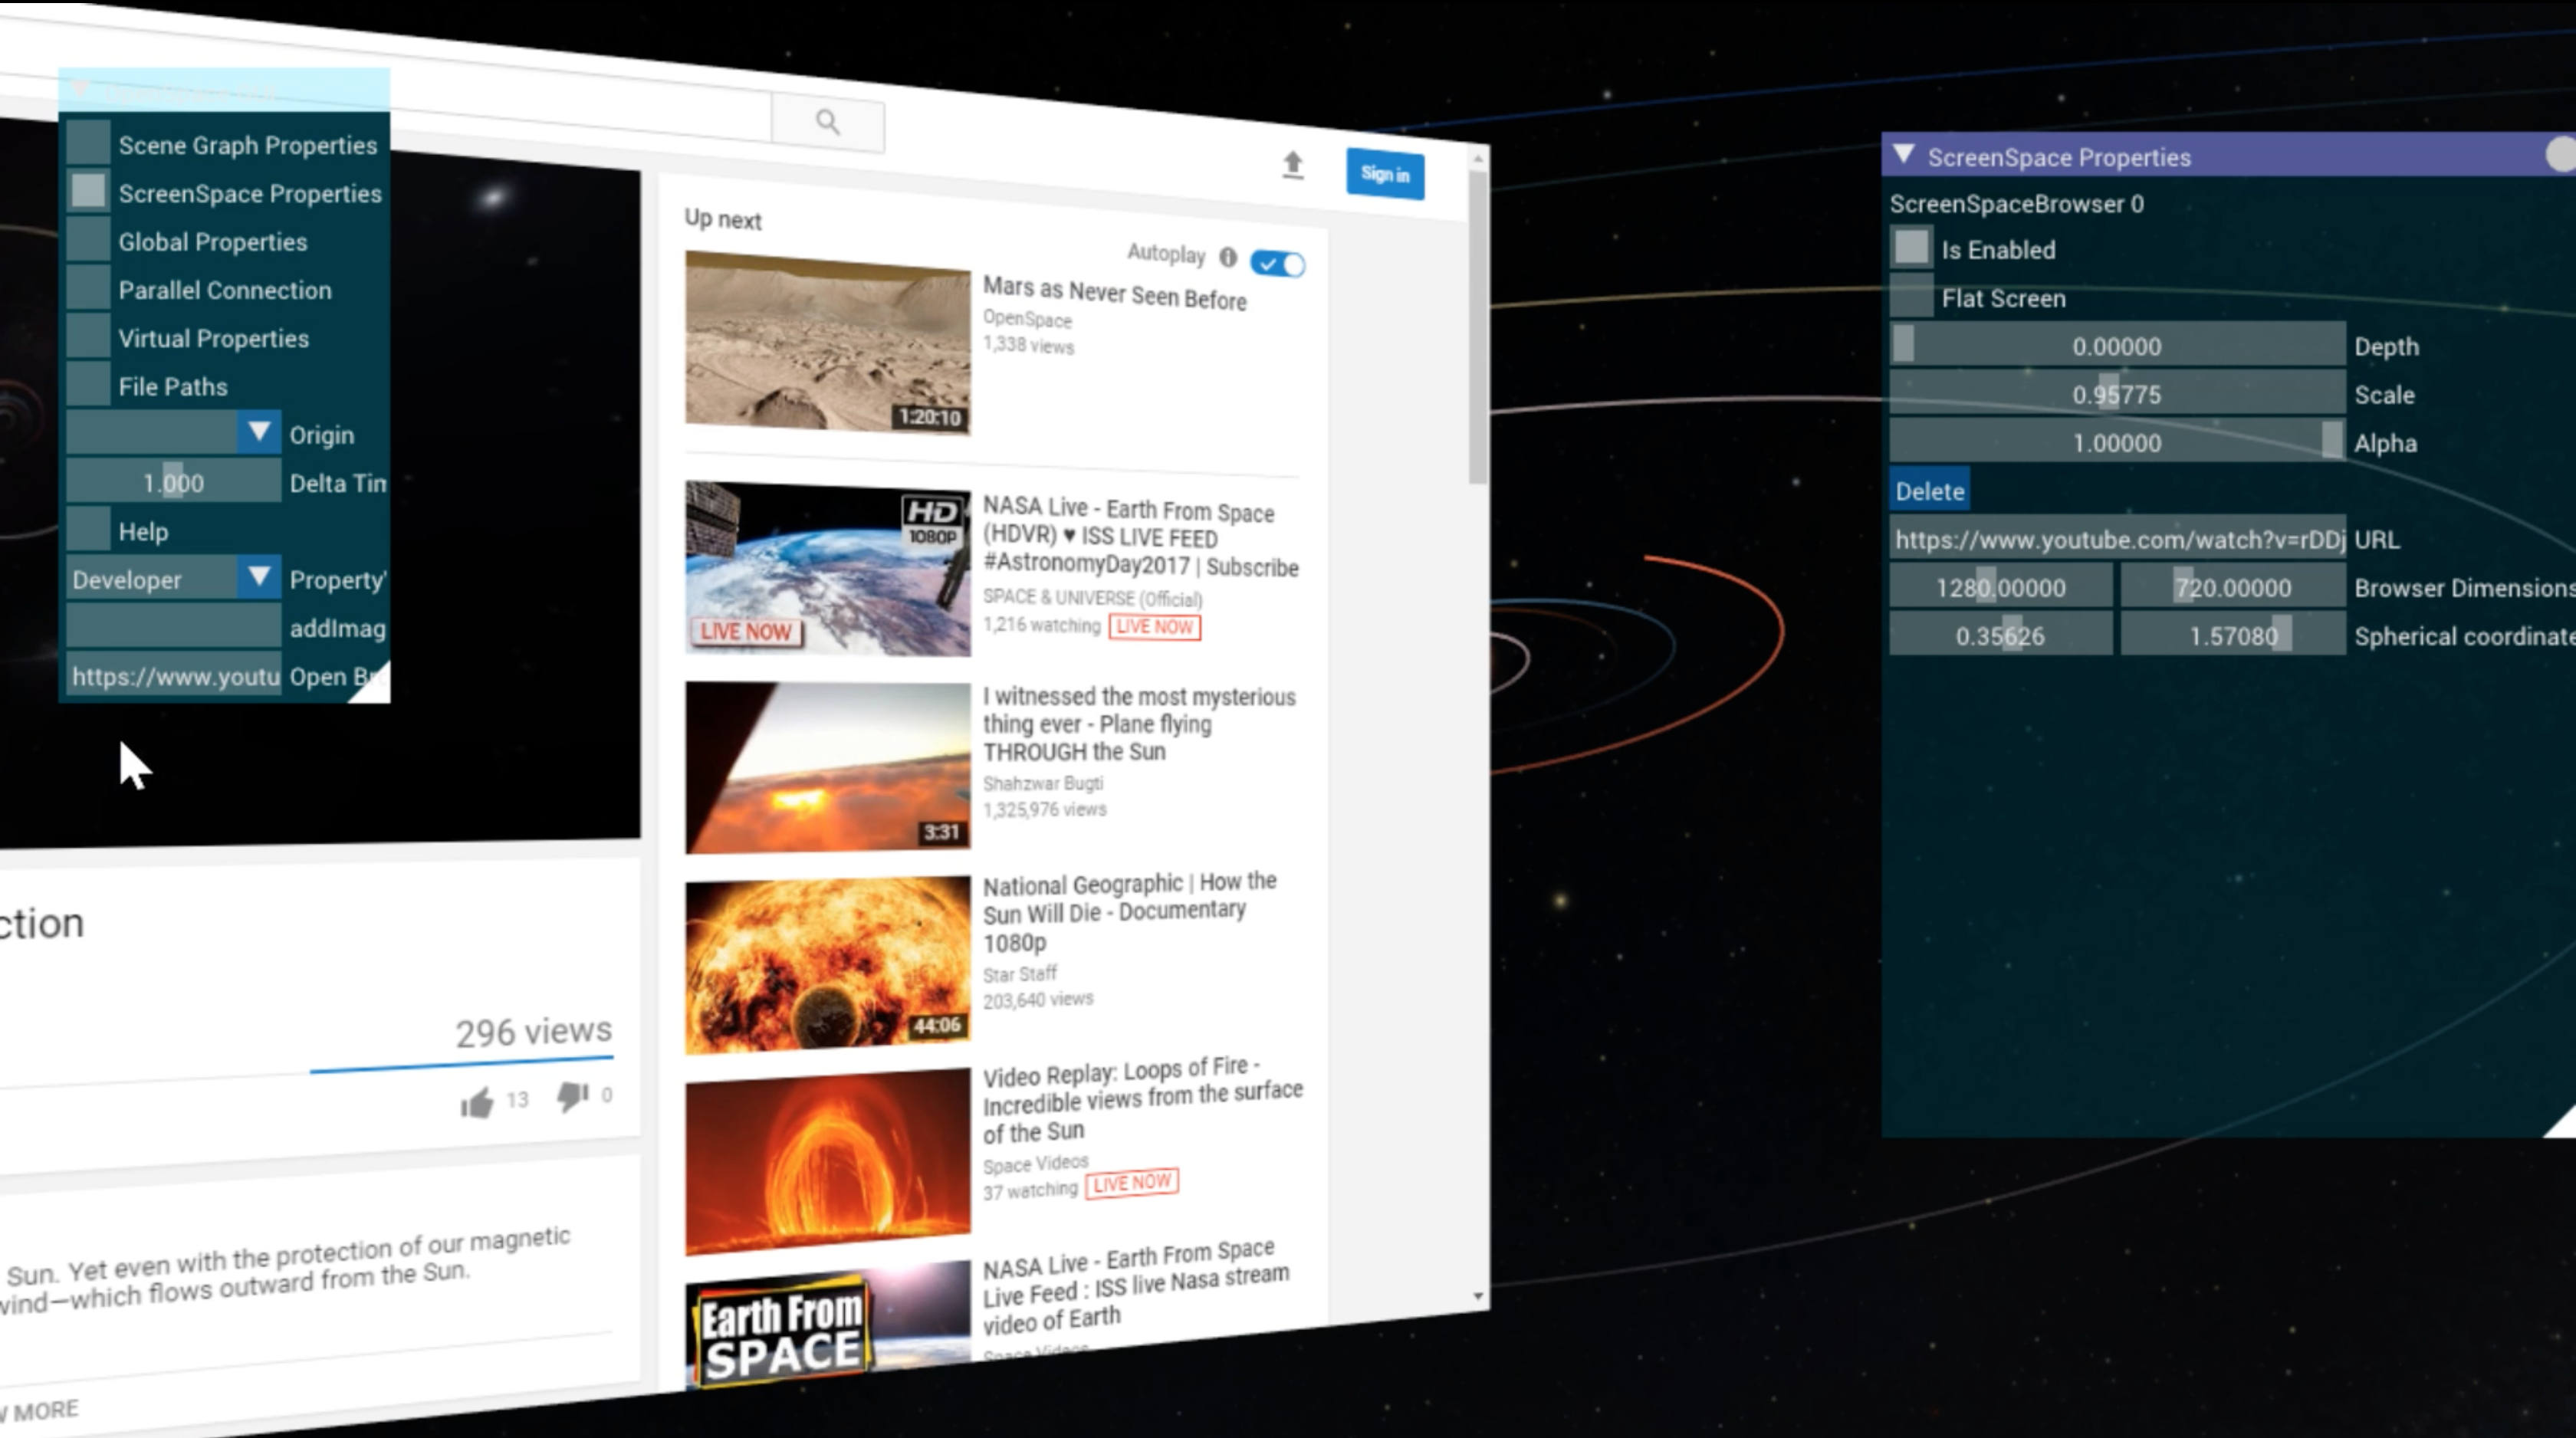
\includegraphics[width=0.7\linewidth]{./figures/screenspace.png}
\caption{\emph{The screen space browser with controls. The browser window is showing a video from the Openspace Youtube page.}}\label{fig:screenspace}
\end{figure}

The second is the screen-covering GUI browser. This is a transparent browser layer that covers the entire Openspace window. This is used to render the GUI on screen. See figure \ref{fig:guiprocess} for an early screen shot in the process of creating the GUI. While the screen space browser has a dynamic window size, allowing it to be changed as the user wants, the GUI browser's dimensions change as the window is resized.

\begin{figure}[!h]
\centering
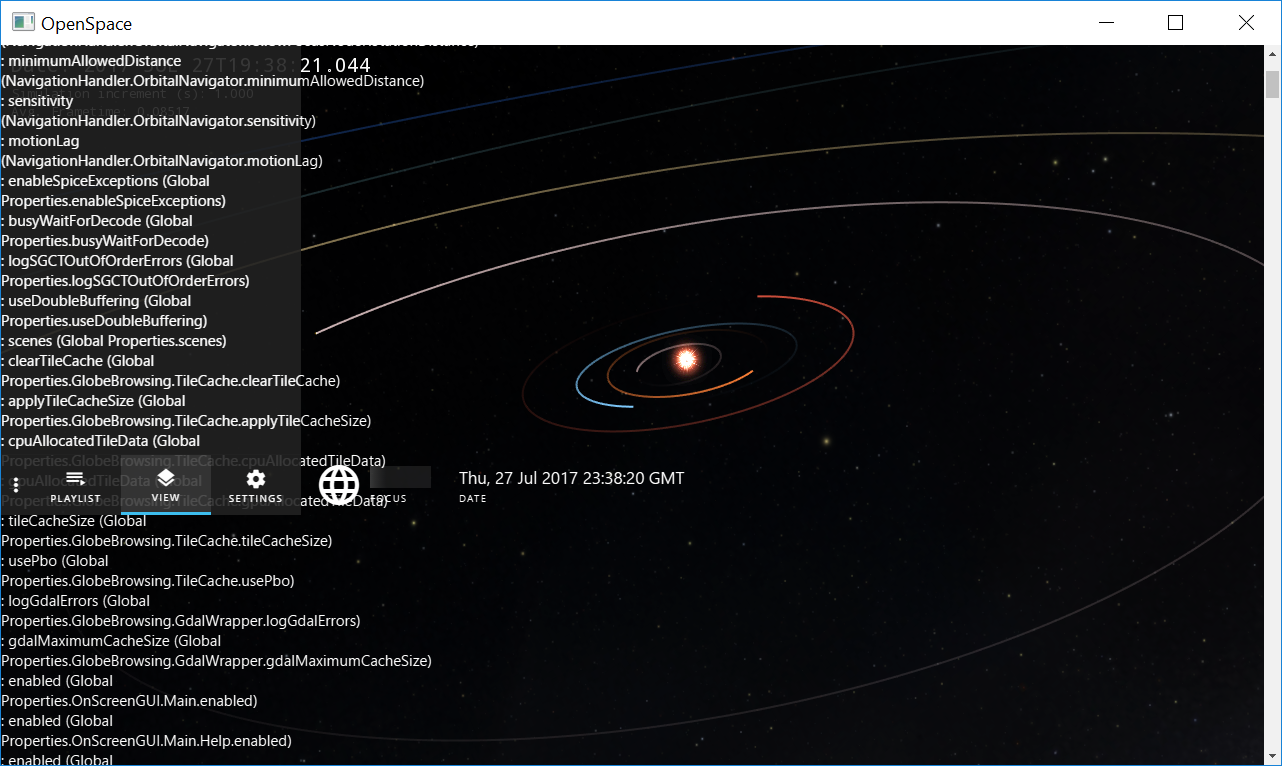
\includegraphics[width=0.7\linewidth]{./figures/guiprocess.png}
\caption{\emph{A screen shot from the GUI development, showing a misaligned sidebar and stringified JSON response from the simulation.}}\label{fig:guiprocess}
\end{figure}

\subsection{Event handling and interaction}\label{sec:interaction}

To handle events and interactions from the user, an event handler was created. This is a C++ class that holds a reference to a single active browser window within Openspace. This can be either a screen space window or the GUI window. This event handler listens to the events that gets captured by Openspace, which include keyboard button clicks, mouse movement, mouse button clicks and mouse scroll wheel movement. These get sent to the active browser windows using corresponding public methods.

To determine whether or not a mouse event should be captured, and blocked from triggering other parts of Openspace, a transparency layer mask is stored by each browser window. This is based on the assumption that an interaction over a transparent area won't trigger anything on the web page. See figure \ref{fig:maskweb} for an example view in the GUI and figure \ref{fig:maskmask} for its corresponding layer mask.

\begin{figure}[!h]
  \centering
  \subfloat[The GUI as it looks in Openspace, overlooking the surface of Mars.]{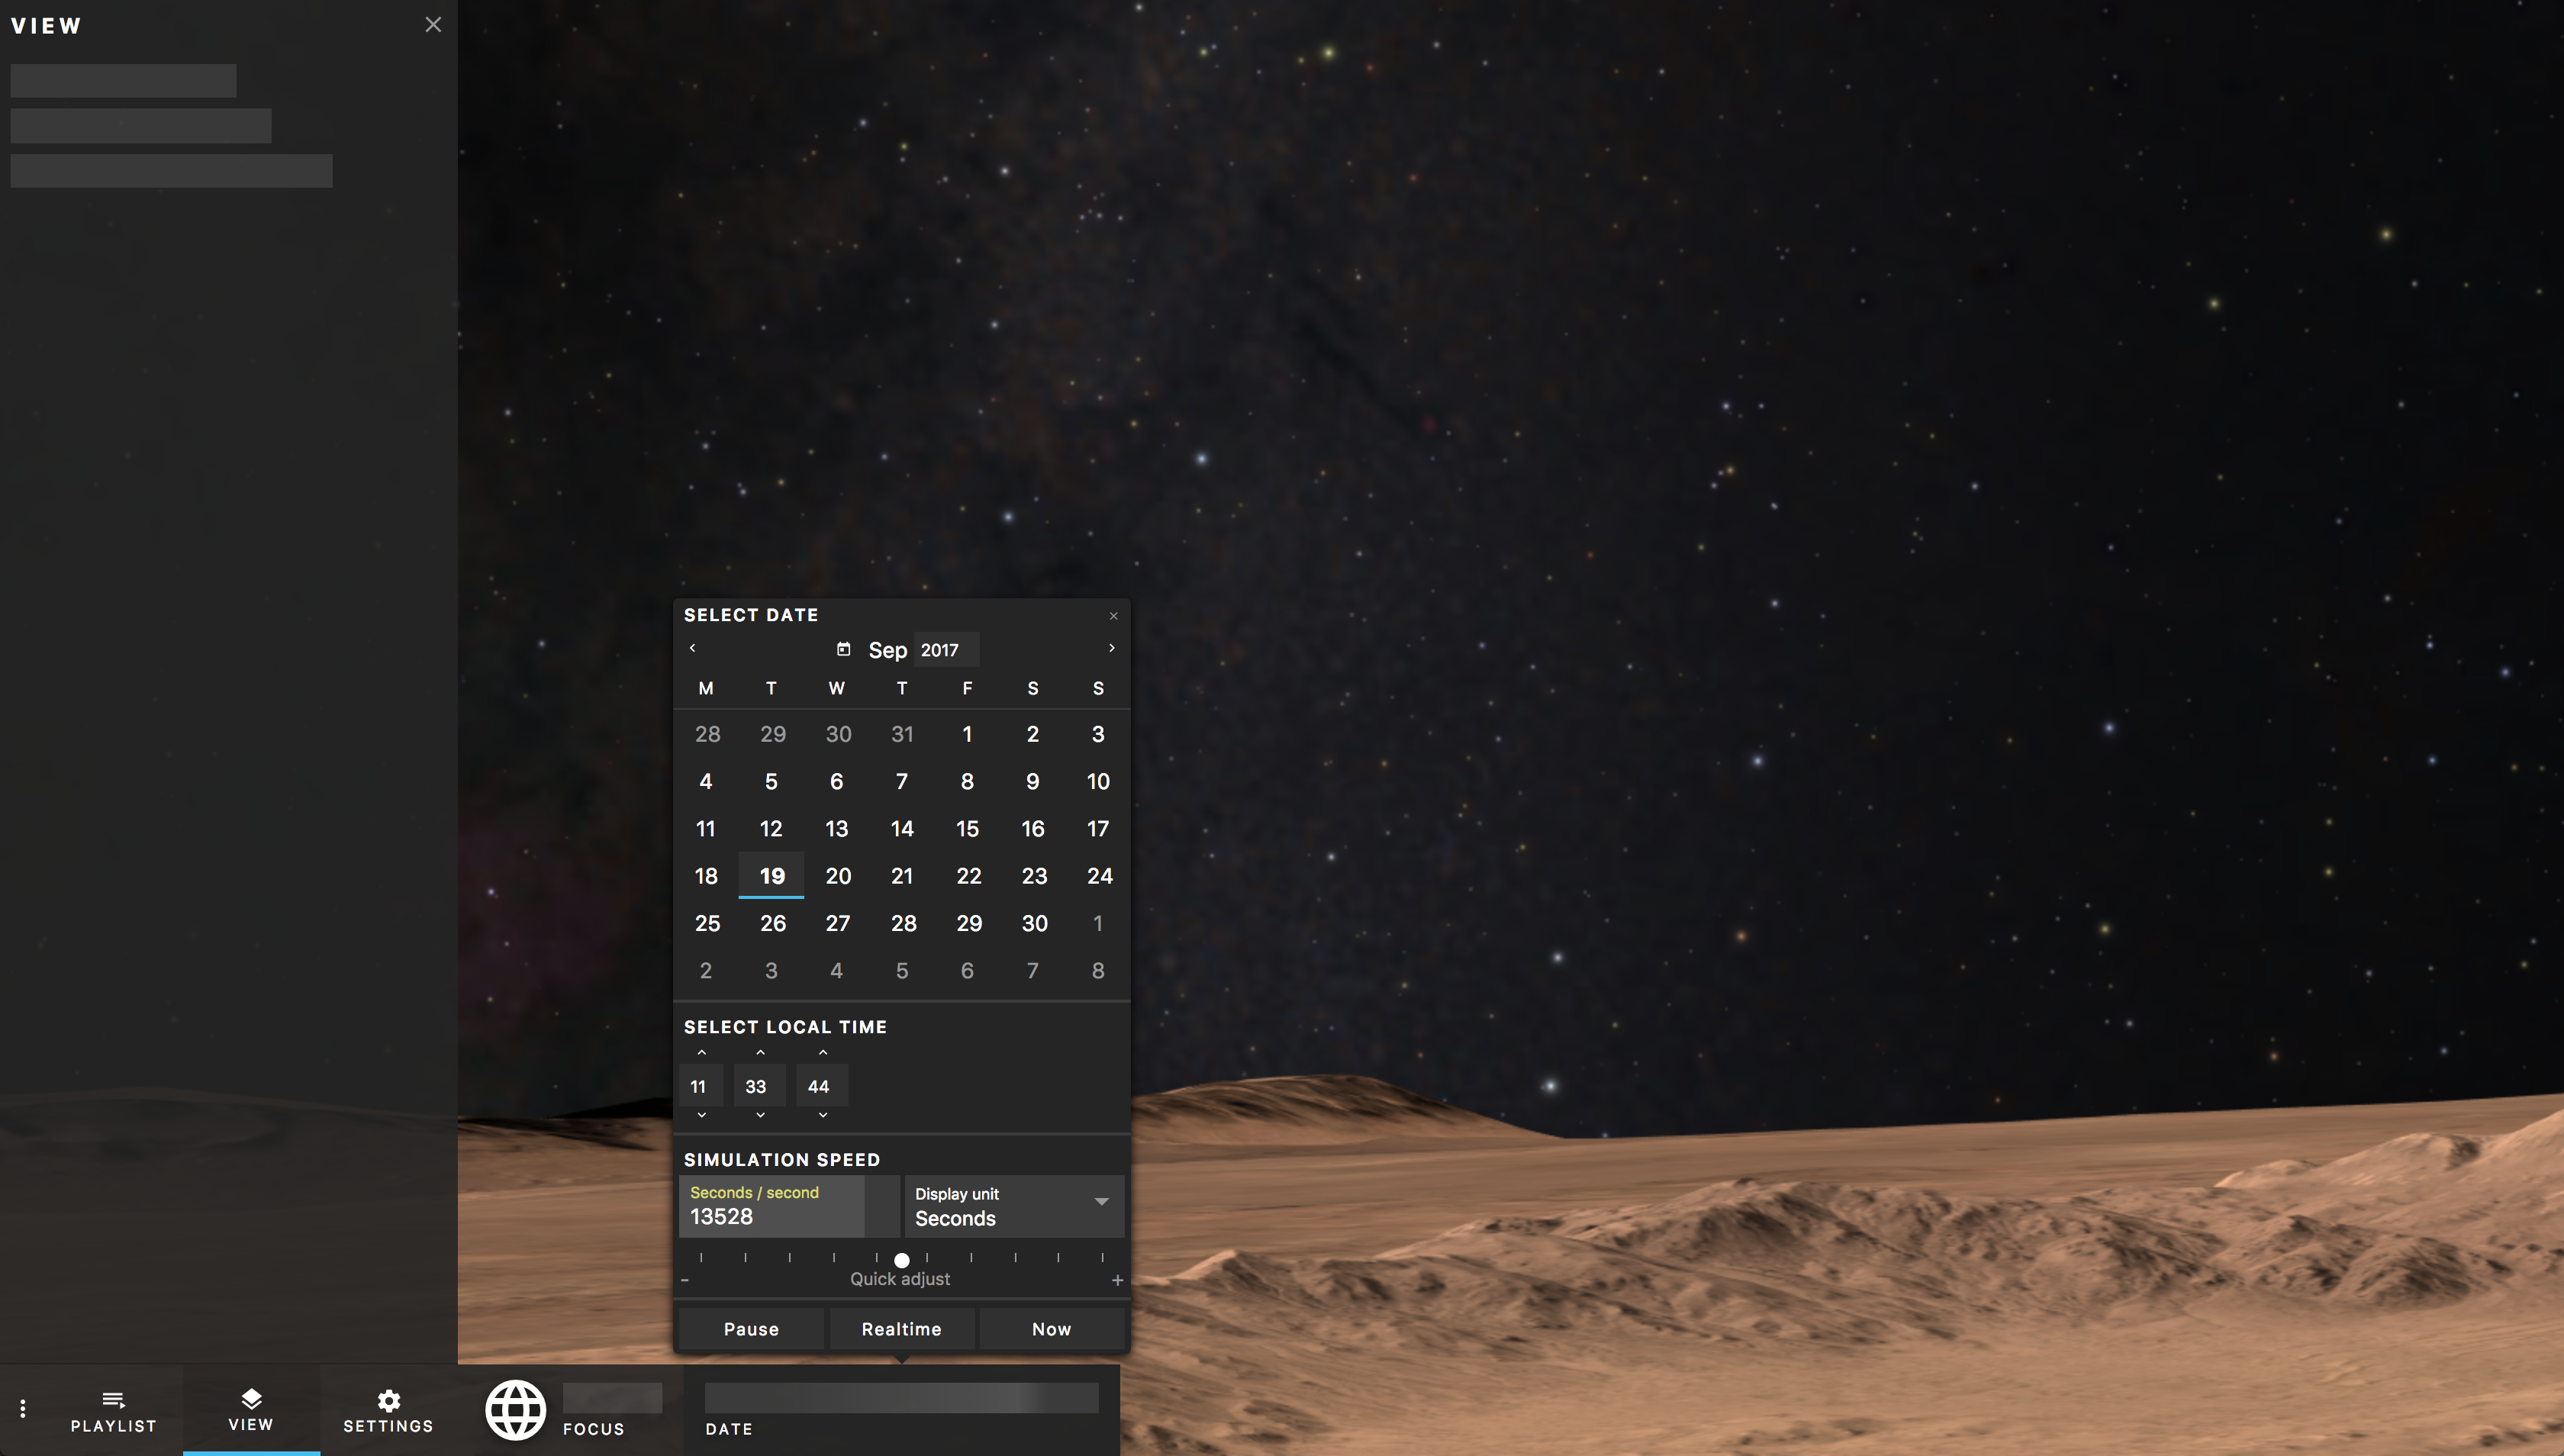
\includegraphics[width=0.45\textwidth]{./figures/maskweb.png}\label{fig:maskweb}}
  \hfill
  \subfloat[The layer mask. The black area will capture mouse clicks and mouse wheel movement.]{\fbox{
\includegraphics[width=0.45\textwidth]{./figures/maskmask.png}\label{fig:maskmask}}}
  \caption{The layer interaction mask}
\end{figure}

The layer mask is stored as a one-dimensional C++ array, and is updated every time the GUI is re-rendered. See more about the rendering in section \ref{sec:rendering}. When a user clicks inside the area marked as non-transparent, this will be sent to the GUI, and the event is captured. If the user clicks outside the area, the event will be ignored by the GUI, and the event trickles on within Openspace.

To get the index $i$ in the one-dimensional layer mask array from the coordinates $x$ and $y$, equation \ref{eq:coordtoidx} is used. Here, $W$ is the width of the browser window. This equation is used to decide whether or not the user's interaction is within an active area of the browser or not, as the position is given as coordinates in Openspace's event handlers.

\begin{equation}\label{eq:coordtoidx}
  i = x + y \cdot W
\end{equation}

\todo{figure with hit and miss on mask? is it needed?}

Keyboard button events, typing, is always sent to the GUI and never blocked. The phenomena caused by this, such as keyboard shortcuts getting unintentionally triggered, will later be discussed. \todo{discuss double effects of some key presses}

\begin{figure}[!h]
\centering
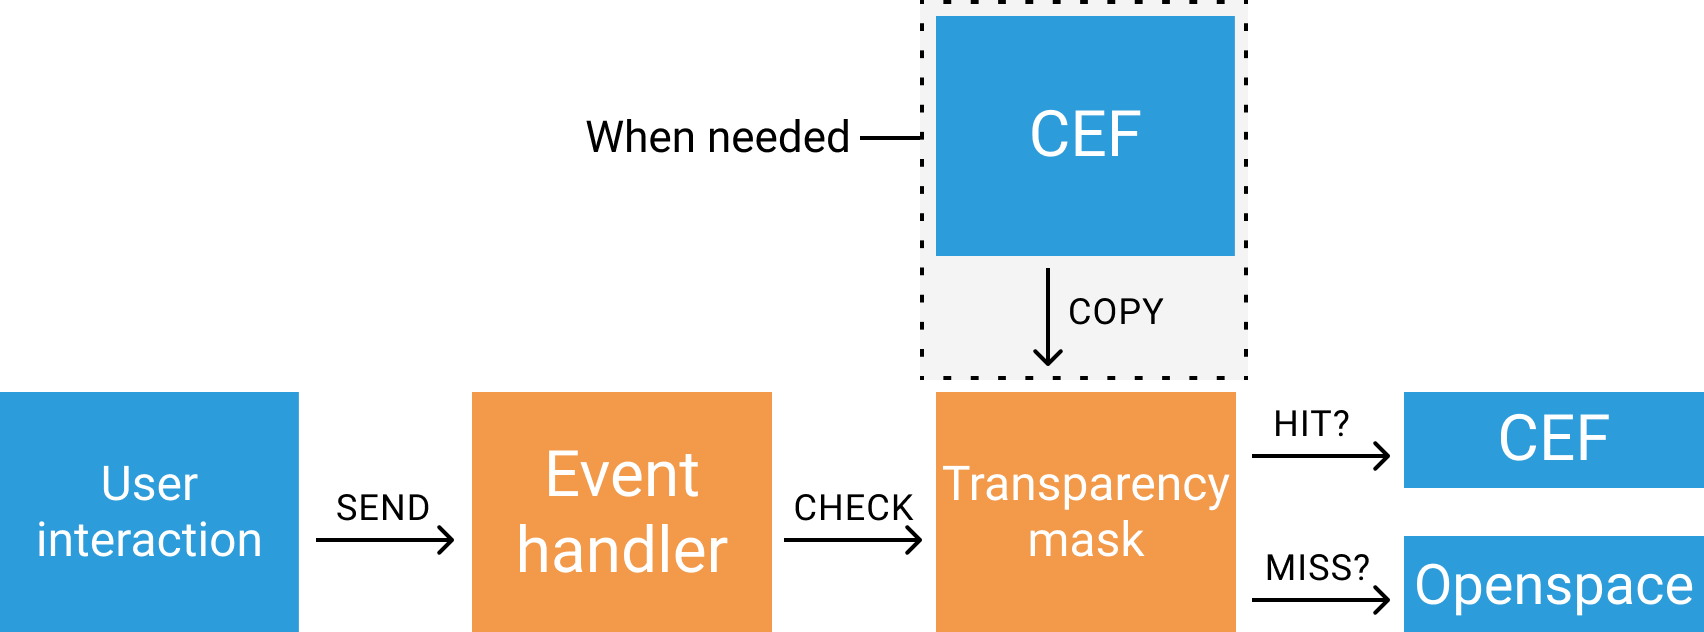
\includegraphics[width=0.9\linewidth]{./figures/maskupdate.png}
\caption{\emph{Overview of the mask update and user interaction process.}}\label{fig:maskupdate}
\end{figure}

When a browser window gets repainted, a buffer stored in the web renderer gets updated, see \ref{sec:rendering}. At this time, the layer mask also gets updated. To do this, the alpha channel of the RGBA values are extracted. If the alpha value of a pixel is non-zero, meaning that it is untransparent, this is considered a pixel that will capture the mouse events. See the life cycle of the interaction decision process in figure \ref{fig:maskupdate}.

\subsection{Rendering}\label{sec:rendering}

\begin{figure}[!h]
\centering
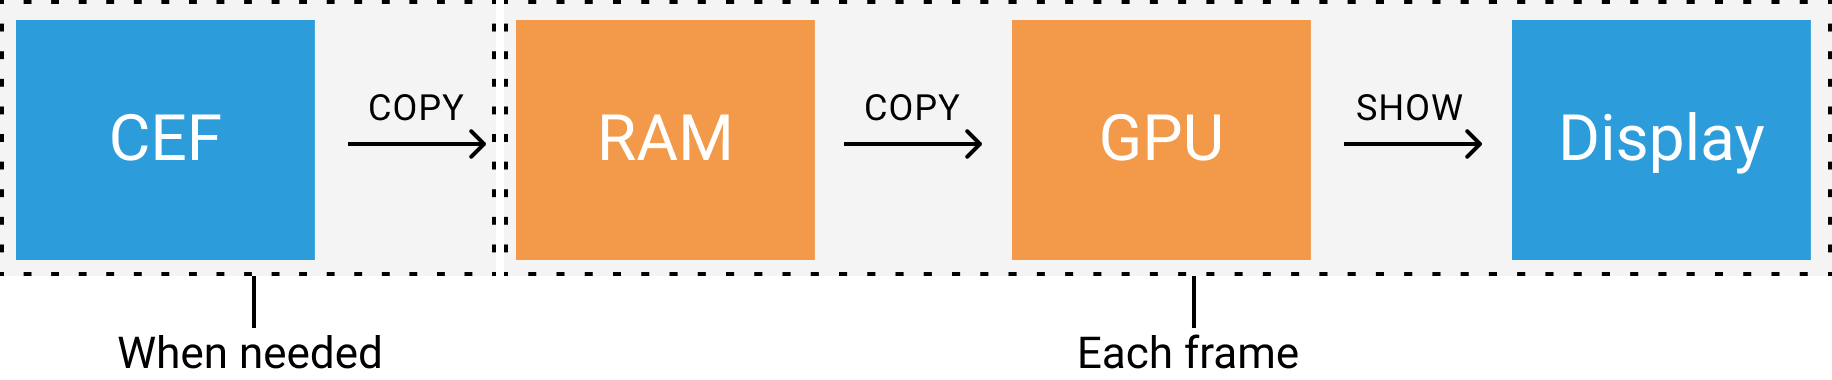
\includegraphics[width=0.9\linewidth]{./figures/rendering.png}
\caption{\emph{Overview of the rendering process.}}\label{fig:rendering}
\end{figure}

The rendering is a two-part process. First, CEF renders the web page to a buffer. This buffer is then copied on the working memory from CEF to the web browser implementation in Openspace. The buffer is then copied, each frame, to the GPU in the OpenGL pipeline in order to be drawn on the screen. The copying from CEF to Openspace is triggered only when the web page needs to be rendered, and the stored buffer is used until it gets updated and replaced by a new copy. See figure \ref{fig:rendering} for an overview of the steps in the rendering process.

To reduce the computing power needed, CEF only updates the buffer when something on the web page gets changed and a repaint of the web page is needed. This can be a colour changing, text changing, box moving or anything similar. Regardless of the magnitude of the change or the cause of this change, the whole buffer gets replaced. This affects both the transparency mask mentioned in section \ref{sec:interaction} and the buffer that gets copied to the GPU for rendering. Depending on the internal bandwidth of the computer, this copying from the RAM to the GPU might be a time consuming task, affecting the performance of the simulation. The implications of this will be discussed later. \todo{discuss ram to gpu copying}

\section{Socket server and simulation control}

To make sure that the simulation actually was controllable from the GUI, ways of communicating between the simulation and the GUI needed to be put into place. This was done by implementing a web socket server within Openspace. The GUI and socket server send JSON messages back and forth with instructions and information. An example request can be seen in listing \ref{lst:request}.

\begin{lstlisting}[caption={Example request sent by the GUI},label=lst:request]
{
  "type": "example",
  "topic": 1,
  "payload": {}
}
\end{lstlisting}

There are some element in this JSON body that are needed for each request:

\begin{itemize}
\item \texttt{type} is a string that describes what type of message this is, and should correspond to one of the implemented \emph{Topics} (more on this later),
\item \texttt{topic} is a required numeric identifier for this message and its possible responses, and
\item \texttt{payload} is a object containing the message details and has further instructions.
\end{itemize}

A response from the socket server can be seen in listing \ref{lst:response}. Here, the \texttt{type} is no longer needed. The client should be aware of the \texttt{topic}, as there are no messages sent on the server's initiative.

\begin{lstlisting}[caption={Example request sent by the GUI},label=lst:response]
{
  "topic": 1,
  "payload": {}
}
\end{lstlisting}

\subsection{Types of requests and responses}

The different types of requests are called topics. There are a number of different types, each with a separate purpose. The implemented topics are:

\begin{itemize}
  \item \emph{authorize}, used to authorize a connection,
  \item \emph{bounce}, a ping-like mechanism, that simply bounces back a response,
  \item \emph{get}, get the value of a given \emph{property},
  \item \emph{lua script}, run arbitrary Lua scripts in the Openspace environment,
  \item \emph{set}, set the value of a given \emph{property},
  \item \emph{subscription}, subscribe to the value of a given \emph{property},
  \item \emph{time}, various special-case time related operations, and
  \item \emph{trigger}, trigger a \emph{trigger property}.
\end{itemize}

The \emph{properties} mentioned in the list above are Openspace properties that may be attached to an object. These objects can for instance be groups of settings, a planet in the scene or the stars in the background. Each property has a URI-like key parameter, that may describe which object it belongs to and what this specific property is named. There are also different types of properties; string, numeric, boolean, trigger, vector and matrix. An overview of the property sending mechanism can be seen in figure \ref{fig:propertysending}. \todo{consider moving this to theory?}

\begin{figure}[!h]
\centering
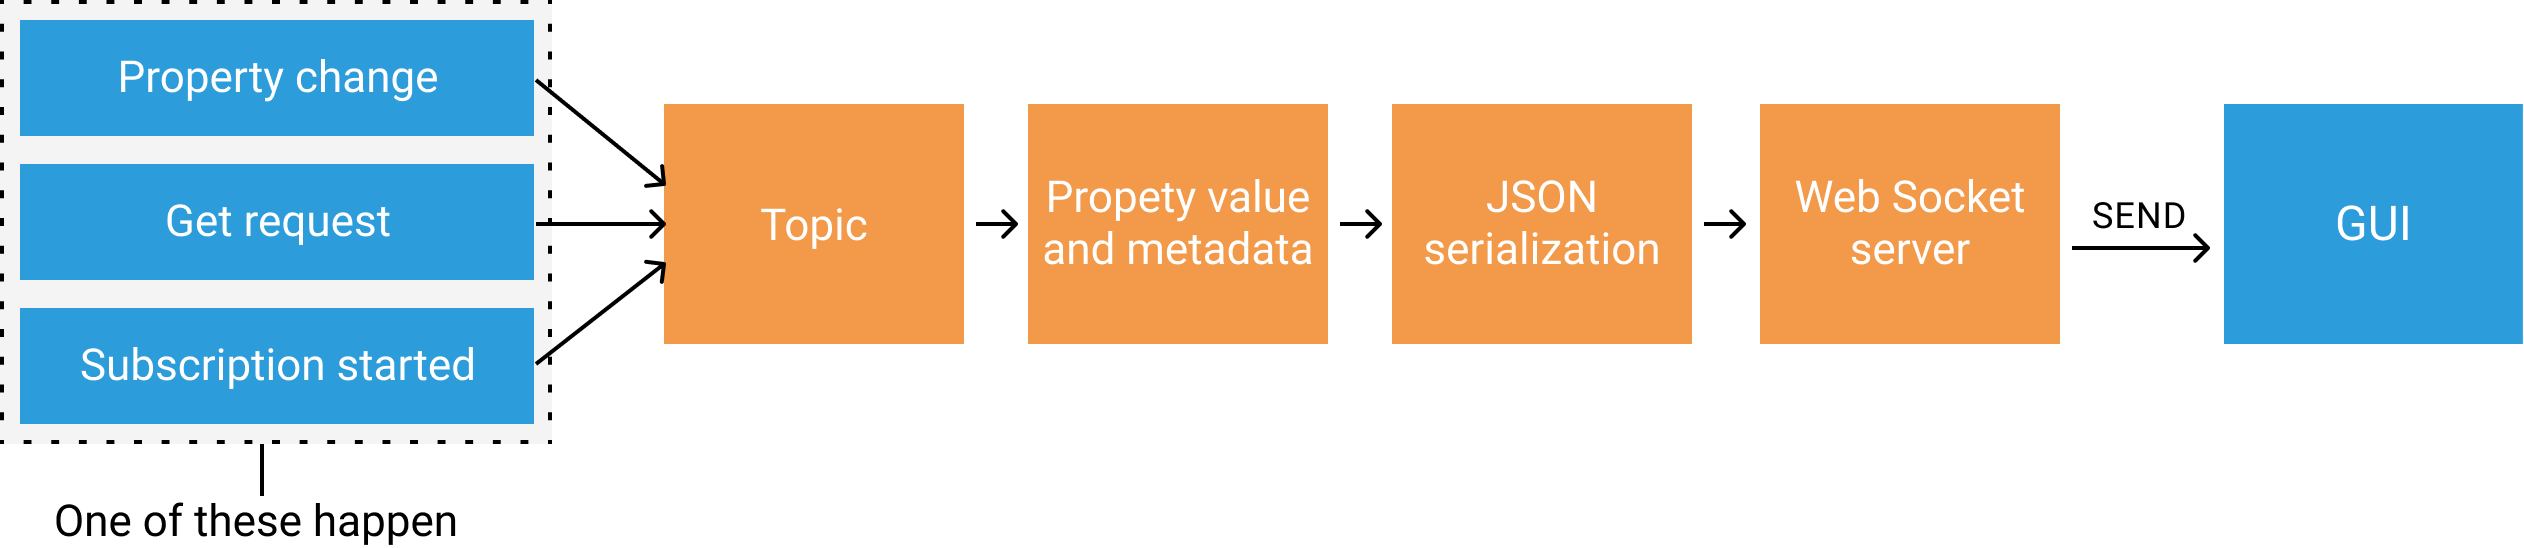
\includegraphics[width=0.9\linewidth]{./figures/propertysending.png}
\caption{\emph{Overview of the property sending mechanism.}}\label{fig:propertysending}
\end{figure}

The payloads of each topic varies. Every topic have different purposes, but some of them have similarities. To use the topics \emph{get}, \emph{set}, \emph{subscribe} or \emph{trigger}, the payload always contain the key-value-pair \texttt{property}. This should contain the URI-like key of the wanted property. See listing \ref{lst:getreq} for a \emph{get} topic request. In this example, \emph{get} could be changed to any of \emph{subscribe} or \emph{trigger} and still be a valid request. The purpose of that request would simply be different.

\begin{lstlisting}[caption={Example get request sent by the GUI},label=lst:getreq]
{
  "type": "get",
  "topic": 1,
  "payload": {
    "property": "example"
  }
}
\end{lstlisting}

On a \emph{get} request, the client asks for the value of the named property. The server receives the request, and if the named property can be found, a message is sent back to the client with the property in a JSON formatted structure. The serialization will be further explained later. On a \emph{subscription} request, the client asks to be notified each time the value of the given property has changed. If the server finds the given property, a callback that gets called each time the property changes it's value gets inserted. This callback sends the message to the client, just like the \emph{get} requests. A copy of the current value also gets sent immediately. The \emph{trigger} requests work differently. Here, no message gets sent back to the client, as the trigger property itself has no value. It can be thought of as a button. Pressing the button has no value itself - it is the underlying mechanisms that cause something to happen. This, in turn, could potentially be subscribed to or retrieved. To use the \emph{set} property, the client also needs to provide a new value to the property. See listing \ref{lst:setreq} for an example set request, where a three dimensional vector property gets set to \texttt{[1, 2, 3]}. \todo{add figure for property changing}

\begin{lstlisting}[caption={Example get request sent by the GUI},label=lst:setreq]
{
  "type": "set",
  "topic": 1,
  "payload": {
    "property": "example",
    "value": [1, 2, 3]
  }
}
\end{lstlisting}

To verify that the client actually should get access to the web socket server, the \emph{authorize} topic exists. This can be used to prove the client's validity by providing a password. Whether or not this is required can be set in the Openspace configuration file, along with the password and an optional list of whitelisted IP addresses. The clients connecting from an IP address in the whitelist will not need authorization. If the client is not from one of the white listed addresses, however, all the topic requests but \emph{authorize} are disregarded until the client is considered authorized. In listing \ref{lst:authreq} for an example request. In listing \ref{lst:authrespok} a message telling the client it is authorized is shown. Listing\ref{lst:authrespnope} shows the message sent when the client could not be authorized. The code entry in the responses mimics HTTP status codes, see \cite[ch. 10]{RFC2616}.

\begin{lstlisting}[caption={Example authorization request sent by the GUI},label=lst:authreq]
{
  "type": "authorize",
  "topic": 1,
  "payload": {
    "key": "example-password"
  }
}
\end{lstlisting}

\begin{lstlisting}[caption={Example authorization granted response sent by the server},label=lst:authrespok]
{
  "message": "Authorization OK.",
  "code": 200
}
\end{lstlisting}

\begin{lstlisting}[caption={Example authorization denied response sent by the server},label=lst:authrespnope]
{
  "message": "Invalid key.",
  "code": 401
}
\end{lstlisting}

The \emph{bounce} topic provides a ping-like mechanism. Immediately when the server receives a bounce request, it sends back a bounce response. The \texttt{payload} sent may contain anything and is returned to the client.

The \emph{lua script} topic allows the client to send an arbitrary lua script that will be executed by Openspace. This can for instance be shutting down the application or similar. There is no responses being sent back. An example request can be seen in listing \ref{lst:luareq}.

\begin{lstlisting}[caption={Example Lua script request sent by the GUI, toggling the shut down process in OpenSpace.},label=lst:luareq]
{
  "type": "luascript",
  "topic": 1,
  "payload": {
    "script": "openspace.toggleShutdown()"
  }
}
\end{lstlisting}

The \emph{time} topic handles everything related to the simulation time. This covers both the speed of the simulation and the actual simulation date and time. The client can subscribe to these items, and change them using the \emph{set} topic. Neither the simulation speed or the date are stored as properties, so to subscribe to them another method is used. By inserting a post render callback into the Openspace engine, the server can see if a value has been changed since it was sent last time. The structure of this request looks much like the \emph{get} request, as seen in listing \ref{lst:getreq}. However, the \texttt{property} entry has the value \emph{currentTime} or \emph{deltaTime}, depending on what callback you want. An example message sent from the server to the client can be seen in listing \ref{lst:timeresp}.

\begin{lstlisting}[caption={Example response for the time topic, sending the current simulation time.},label=lst:timeresp]
{
  "topic": 1,
  "payload": "2017-09-21T10:57:25.123"
}
\end{lstlisting}

The simulation time is expected to change at a high rate. To limit the burden of sending messages, the rate is throttled. This is done on a per-topic basis, requiring a given time to pass between each message.

\subsection{JSON serialization}

As mentioned before, messages sent back and forth between the server and client are JSON formatted. On the server, this is done by using a JSON library that allows arbitrary C++ types to be serialized to JSON. See \cite{jsonlib} for more details on the library. Using this method, nested data structures may be serialized as the library uses recursion.

A serialized Openspace property contains information that describes how it should be handled by the GUI. What type of data it contains, limits, name, description and its value are described. See listing \ref{lst:jsonproperty} for a completely serialized property.

\begin{lstlisting}[caption={},label=lst:jsonproperty]
{
  "Value": 123,
  "Description": {
    "description": "Example description, explaining this property to the user",
    "Type": "The type of this property",
    "Identifier": "The URI to this property",
    "Name": "The name to show in the GUI",
    "MetaData": {
      "Group": "",
      "Visibility": "All", // one of All, Developer, User and Hidden
      "ReadOnly": false
    },
    "AdditionalData": {}
  }
}
\end{lstlisting}

\section{GUI}

\include{discussion}
\include{conclusion}
\printbibliography

\end{document}

%%%%%%%%%%%%%%%%%%%%%%%%%%%%%%%%%%%%%%%%%%%%%%%%%%%%%%%%%%%%%%%%%%%%%%
%%% demothesis.tex ends here

